\documentclass[9pt,twocolumn,twoside]{../../styles/osajnl}
\usepackage{fancyvrb}
\usepackage[colorinlistoftodos,prependcaption,textsize=normal]{todonotes}
\newcommand{\TODO}[2][]{\todo[color=red!10,inline,#1]{#2}}
\newcommand{\GE}{\TODO{Grammar}}
\newcommand{\SE}{\TODO{Spelling}}
\newcommand{\TE}{\TODO{Term}}
\newcommand{\CE}{\TODO{Citation}}
\journal{i524} 

\title{Google Dremel: SQL-Like Query for  Big Data}


\author[1,*]{Jimmy Ardiansyah}

\affil[1]{School of Informatics and Computing, Bloomington, IN 47408, U.S.A.}


\affil[*]{jardians@indiana.edu - S17-IR-2002}

\dates{Research Article-01, \today}

\ociscodes{Google Dremel, Big Data Query }

% replace this with your url in github/gitlab
\doi{\url{https://github.com/jardians/sp17-i524/tree/master/paper1/S17-IR-2002/report.pdf}}
 
\begin{abstract}
Dremel is a scalable, interactive ad-hoc query system for analysis of
read-only nested data. By combining multi-level execution trees and
columnar data layout, it is capable of running aggregation queries
over trillion-row tables in seconds.\newline
\end{abstract} 
   
\setboolean{displaycopyright}{true} 

\begin{document}

\maketitle

\TODO{This review document is provided for you to achieve your
  best. We have listed a number of obvious opportunities for
  improvement. When improving it, please keep this copy untouched and
  instead focus on improving report.tex. The review does not include
  all possible improvement suggestions and for each comment you may
  want to check if it applies elsewhere in the document.}

\TODO{Please, use 80 character lines in the LaTeX source. Makes
  reading the paper easier.}

\TODO{Abstract: Good. It can be expanded with another sentence or two
  with examples of tasks it has been used for.}

\TODO{Overall, you do a good job of explaining what Dremel is and how
  it works. However, the parts of the paper that have to give a more
  general idea about Dremel (intro and conclusion for example) need to
  be written in a more neutral voice. That is, you need to tone down
  some of the superlative words you are using like "drastically",
  "super", "unprecedented" and so on. The goal of the paper is to
  inform about specific qualities of Dremel in a neutral way, and
  backing up claims with citations. The use of words like these is not
  appropriate for a paper like this, even in sections that are aimed
  at providing a broader view of Dremel.}

\TODO{Assessment: Some revisions recommended. Please address the notes
  below by end of March.}

\section{Introduction}
Big data analytics nowadays has become more common across industries
and government agencies partly due to fast and affordable commodity
storage to keep pace with data and business growth.

Make the data sense at the fingertips \TODO{Not clear. Data sense?} of
data scientists and analysts has become increasingly essential to
compete in the business world. Having interactive tool with fast
response times often make \GE a difference in data exploration, rapid
prototyping as well as designing \TE of data pipelines. Performing
interactive data analysis at scale demands a high degree of
parallelism. That's where Dremel comes into play.

Dremel is a scalable, interactive ad-hoc query system for analysis of
read-only nested data. By combining multi-level execution trees and
columnar data layout, it is capable of running aggregation queries
over trillion-row tables in seconds.  The system scales to thousands
of CPUs and petabytes of data.  With Dremel, you get to write a
declarative SQL-like query against data stored in a very efficient for
analysis read-only columnar format. It's also possible to write
queries that analyze billions of rows, terabytes of data, and
trillions of records in seconds ~\cite{paper-dremel}.

\section{History Development}

\TODO{This section mixes the historical development with elements from
  the architecture of Dremel (column store, definition and repetition
  levels, reconstructing a record, etc.). This will better serve as
  the first two paragraph of the architecture section.}

When Google published the Dremel paper in 2010, it explained how this
structure is preserved within column store. Every column, in addition
to its value, also stores two numbers — definition and repetition
levels.

This encoding ensures that the full or partial structure of the record
can be reconstructed by reading only requested columns, and never
requires reading parent columns (which is the case with alternative
encoding). That same paper gives an exact algorithm for both encoding
the data and reconstructing the record.

In 2014, Google published another paper — Storing and Querying
tree-structured records in Dremel \TODO{Please use a citation. You
  don't need to include the title of the paper in the text if you cite
  it.} — which lays theoretical foundation and proves correctness of
algorithms for filtering and aggregation operators, which take
advantage of the above encoding.~\cite{www-dremel}.

\section{Why Dremel} \TODO{Needs question mark.}

This observation report discusses some characteristics of Dremel; a
system that supports interactive analysis of very large datasets over
shared clusters of commodity machines. \TODO{This first sentence is
  not necessary. You've already discussed what Dremel is at a high
  level, and you should try to avoid focusing on the paper (e.g. "This
  observation report discusses...") and focus on Dremel itself.}
Dremel can even execute a complex regular expression text matching on
a huge logging table that consists of about 35 billion rows and 20 TB,
in merely tens of seconds. \TODO{This is a very specific statement
  that needs a reference. Also, why focus on something so specific in
  a general "Why Dremel?" section?} This is the power of Dremel; it
has super high \TODO{"super high" is subjective and too conversational
  for a paper like this} scalability and most of the time it returns
results within seconds or tens of seconds no matter how big the
queried dataset is.  Why Dremel can be as drastically
\TODO{"drastically" is subjective} fast as the examples show?
\TODO{You need to clarify what examples or remove this sentence. Are
  these related to something you've discussed in the paper so far, or
  of the references? It is not clear.} The answer can be found in two
core technologies which gives Dremel this unprecedented
\TODO{"unprecedented" is subjective;} performance:

\begin{enumerate}
  \item Columnar Storage. Data is stored in a columnar storage fashion
    which makes possible to achieve very \TODO{try to avoid using
      adverbs like "very"} high compression ratio and scan throughput.
  \item Tree Architecture is used for dispatching queries and
    aggregating results across thousands of machines in a few seconds
    ~\cite{paper-dremel}. \TODO{This is more the tone and wording the
      whole paper should use. Still, "across thousands of machines in
      a few seconds" is not very specific so you should see if you can
      make this a little more concrete based on what the paper
      reports}
\end{enumerate}

\subsection{Columnar Storage.}
Dremel stores data in its columnar storage, which means it separates a record into column values and stores each value on different storage volume, whereas traditional databases normally store the whole record on one volume; this is efficient for cases where many columns of the records need to be fetched. For example, if one analysis heavily relied on fetching all fields for records that belong to a particular time ranged, row-oriented storage would make sense. 

To illustrate what columnar storage is all about, here is an example with three columns

\begin{figure}[H]
 \centering
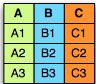
\includegraphics[scale=0.7]{images/image1}
\caption{Typical row-oriented storage}
\end{figure}

In a row-oriented storage, the data is laid out one row at a time as
follows: \TODO{When you write a paper like this, it is best not to
  assume where a figure will be placed on the page. Thus, don't use a
  colon, but say "In Figure\\ref\{...\}, ...". This is for two
  reasons: 1) Paper formats differ between different conferences and
  journals, so you're not guaranteed where a figure will be placed. 2)
  LaTeX itself doesn't always guarantee exact placement on the page.}

\begin{figure}[H]
 \centering
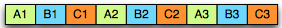
\includegraphics[scale=0.7]{images/image2}
\caption{Transform row to column-oriented format}
\end{figure}

Whereas in a column-oriented storage, it is laid out one column at a
time: \TODO{See above about using the colon/assuming where the figure
  will appear on the page.}

\begin{figure}[H]
 \centering
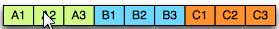
\includegraphics[scale=0.7]{images/image3}
\caption{Laid out the column}
\end{figure}

Dremel has introduced columnar storage, which provides several
advantages over row-oriented system:

\begin{itemize}
  \item Is generally very efficient in term \GE of compression on
    columns because entropy within a column is lower that entropy
    within a block of rows. in other words, data is more similar
    within the same column, than it is in a block of rows. This can
    make a huge \TODO{"huge" is subjective, just use "big"} difference
    especially when the column has few distinct value. \GE
  \item Work well for queries that only access a small subset of
    columns.
  \item I/O will be reduced as we can efficiently scan only a subset
    of the columns while reading the data. Better compression also
    reduces the bandwidth required to read the input.
  \item Is often well suited for data-werehousing applications where
    users want to aggregate certain columns over a large collection of
    records.
  \item As we store data of the same type in each column, we can use
    encoding better suited to the modern processors’ pipeline by
    making instruction branching more predictable
    ~\cite{book-hadoop-apps}.
\end{itemize}

\TODO{This is a nice list of advantages, but please try to provide
  references about some of the assertions in the first four bullet
  points.}

\subsection{Tree Architecture}
Dremel builds on ideas from web search and parallel DBMSs. First, its
architecture borrows the concept of a serving tree used in distributed
search engines. \TODO{This will be difficult to understand for someone
  who doesn't know what a serving tree is. Either provide a little
  more explanation, or include a reference.} Just like a web search
request, a query gets pushed down the tree and is rewritten at each
step. The result of the query is assembled by aggregating the replies
received from lower levels of the tree. Tree Architecture has enable
Dremel to dispatch queries and collect results across tens of
thousands of machines in a matter of seconds by using the Tree
architecture. \TODO{This is a specific empirical claim so it needs a
  reference.} The architecture forms a massively parallel distributed
tree for pushing down a query to the tree and then aggregating the
results from the leaves at a blazing fast \TODO{"blazing fast" is
  subjective and better suited to an advertisment than a paper like
  this} speed ~\cite{twitter-dremel}. Consider a simple aggregation
query below:

\begin{figure}[H]
 \centering
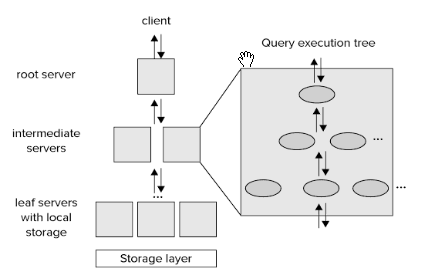
\includegraphics[scale=0.7]{images/image4}
\caption{Typical Tree Architecture ~\cite{book-hadoop}} 
\end{figure}

A root server receives incoming queries, reads metadata from the
tables, and routes the queries to the next level intermediate servers
in the serving tree. The leaf servers communicate with the storage
layer (based on the columnar model described earlier) to read data
which is bubbling up for the aggregation and final result is return to
the user or access the data on local disk.

However, after data is processed, one will be running aggregate
queries and analysis on large chunks of data at a time, most probably
only on a subsets of columns. Because many analytical queries only
select a subsets of columns at a time for storing that will be
analyzed later ~\cite{book-hadoop}.

Overall, Dremel combine \SE parallel query execution with the columnar
format that supporting \TE performance data access and also capable of
operating on in situ \TODO{Use \\emph\{\} to show you are introducing
  a term.} nested data. In situ refers to the ability to access data
'in place', e.g., in a distributed file system like Veritas Cluster
File System, General Parallel File System (GPFS), and Global File
System (GFS). \TODO{Why not simply use "in place" to avoid having to
  explain a new term? Does using "in situ" help understanding in any
  way?}

\section{Implementation of Google Dremel }
Apache Drill is the open source version of Google's Dremel system
which is available as an infrastructure service called Google
BigQuery. One explicitly stated design goal \TODO{Needs
  reference. Where is it stated?} is that Drill is able to scale to
10,000 servers or more and to be able to process petabytes of data and
trillions of records in seconds. \TODO{Specific quantitative claim,
  needs reference.} Drill is an Apache top-level
project. \TODO{Explain briefly what that means (top level project)?}
Drill supports a variety of NoSQL databases and file systems. In
addition, Drill supports data locality, so it's a good idea to
co-locate Drill and the datastore on the same nodes
~\cite{wiki-drill}.

\section{Conclusion}
 Although query and process \GE large volute of data in any system is
 a challenging task, especially in the big data ecosystem due to vast
 expense of option available, Dremel has been standing out as the
 right model \TODO{"standing out as the right model" is subjective}
 for process and storing data with a lot of benefits as well as
 fitting as part of an entire big data stack which can be used against
 raw data, like log data.  Choosing the right tool for your data is
 one of the most important decision one will make in the application,
 and everyone need to spend the appropriate amount of time and effort
 to get it right the first time. \TODO{This sentence is unnecessary.}
 Because of it, I believed \TODO{Don't use "I believe", "I think",
   etc. The paper should have a neutral voice.} Dremel will be the
 future of interactive ad-hoc query system for analysis that require
 fast result. \TODO{Subjective statement.}
 
 \section{Acknowledgements}
this \SE work was done as part of the course "I524: Big Data and Open
Source Software Projects" at Indiana University during Spring 2017


% Bibliography

\bibliography{references}
 
\end{document}

